\documentclass[12pt,a4paper]{article}
% ============================================================================
%  Complete mathematical derivation for the brats-uad latent-diffusion UAD
%  pipeline (KL-VAE + DDPM + DDIM). Overleaf-compatible (pdfLaTeX).
%  All long equations are split across lines to avoid right-margin overflow.
% ============================================================================
\usepackage[utf8]{inputenc}
\usepackage[a4paper,left=22mm,right=22mm,top=20mm,bottom=22mm]{geometry}
\usepackage{amsmath,amssymb,amsthm,mathtools}
\usepackage{bm}
\usepackage{graphicx}
\usepackage{booktabs}
\usepackage{array}
\usepackage{xcolor}
\usepackage{enumitem}
\usepackage{titlesec}
\usepackage{tikz}
\usetikzlibrary{arrows.meta,positioning,calc,fit,backgrounds}
\usepackage{hyperref}
\hypersetup{colorlinks=true,linkcolor=blue!50!black,citecolor=green!50!black,
            urlcolor=red!50!black,pdftitle={brats-uad: Mathematical Derivation}}
\usepackage{times}

% Allow display breaks and keep equations inside the text width.
\allowdisplaybreaks
\setlength{\jot}{6pt} % a little more space between aligned lines

\theoremstyle{definition}
\newtheorem{definition}{Definition}
\theoremstyle{plain}
\newtheorem{theorem}{Theorem}
\newtheorem{proposition}{Proposition}
\newtheorem{lemma}{Lemma}

\newcommand{\R}{\mathbb{R}}
\newcommand{\E}{\mathbb{E}}
\newcommand{\N}{\mathcal{N}}
\newcommand{\KL}{D_{\mathrm{KL}}}
\newcommand{\x}{\bm{x}}
\newcommand{\z}{\bm{z}}
\newcommand{\eps}{\bm{\epsilon}}
\newcommand{\II}{\mathbf{I}}
\newcommand{\abar}{\bar{\alpha}}
\newcommand{\given}{\,\vert\,}
\newcommand{\dd}{\,\mathrm{d}}
\DeclareMathOperator*{\argmin}{arg\,min}
\DeclareMathOperator*{\argmax}{arg\,max}
\DeclareMathOperator{\Var}{Var}
\DeclareMathOperator{\Tr}{Tr}
\DeclareMathOperator{\diag}{diag}

\titleformat{\section}{\normalfont\large\bfseries}{\thesection}{1em}{}
\titleformat{\subsection}{\normalfont\normalsize\bfseries}{\thesubsection}{1em}{}

\title{\textbf{Mathematical Foundations of a Latent-Diffusion Pipeline for\\
Unsupervised Anomaly Detection in Pediatric Brain MRI}\\[3pt]
\large Step-by-step derivations of the KL-VAE, DDPM and DDIM as implemented in
\texttt{brats-uad}, with the project's practical numbers}
\author{Soham Patel \\ \small Deep Vision (Summer 2025) --- OTH Amberg-Weiden}
\date{\today}

\begin{document}
\maketitle
{\small\tableofcontents}
\bigskip

\begin{abstract}
\noindent This document derives, from probability first principles and with every
algebraic step shown, the three generative models that compose the
\texttt{brats-uad} unsupervised anomaly detection (UAD) pipeline: a
\textbf{KL-regularised variational autoencoder} (KL-VAE, 18.2\,M parameters) that
compresses a $4{\times}256{\times}256$ multi-modal MRI slice into a
$4{\times}32{\times}32$ latent ($64\times$ compression); a
\textbf{denoising diffusion probabilistic model} (DDPM) with an 89.5\,M-parameter
UNet that learns the distribution of \emph{healthy} latents; and a deterministic
\textbf{DDIM} sampler that, by partially noising and re-denoising a test latent,
produces a pseudo-healthy counterfactual whose residual localises pathology.
Section~\ref{sec:stats} establishes the statistical machinery (Gaussians,
likelihood, KL divergence, Jensen's inequality, the reparameterisation trick).
Sections~\ref{sec:vae}--\ref{sec:ddim} derive the VAE evidence lower bound, the
diffusion variational bound and its reduction to noise prediction, and the DDIM
update. Section~\ref{sec:score} formalises the scoring, calibration and metrics.
Every model is annotated with the exact hyper-parameters and tensor shapes used
in the code.
\end{abstract}

% ---------------------------------------------------------------------------
\section{The pipeline at a glance}
% ---------------------------------------------------------------------------
The system chains an encoder $E_\phi$, a latent diffusion model $\eps_\theta$, and
a decoder $D_\psi$. Training (the VAE and the diffusion model) sees \emph{only}
healthy anatomy; lesion labels are used solely to \emph{evaluate} the residual.

\begin{figure}[h!]
\centering
\resizebox{\textwidth}{!}{%
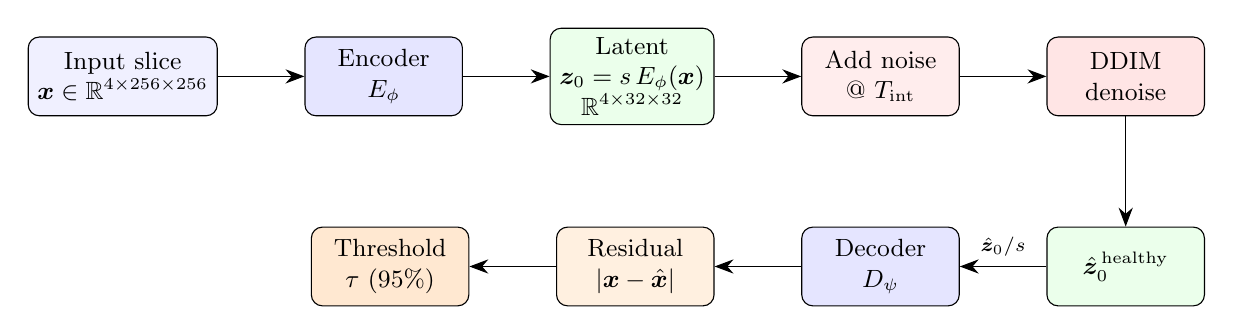
\begin{tikzpicture}[
  node distance=8mm and 11mm,
  box/.style={draw,rounded corners,minimum height=10mm,minimum width=20mm,align=center,font=\small},
  op/.style={draw,circle,inner sep=1pt,font=\footnotesize},
  >={Stealth[length=2.4mm]}]
  \node[box,fill=blue!6]   (x)   {Input slice\\$\x\in\R^{4\times256\times256}$};
  \node[box,fill=blue!10,right=of x] (enc) {Encoder\\$E_\phi$};
  \node[box,fill=green!8,right=of enc] (z0)  {Latent\\$\z_0=s\,E_\phi(\x)$\\$\R^{4\times32\times32}$};
  \node[box,fill=red!7,right=of z0] (noise) {Add noise\\@ $T_{\mathrm{int}}$};
  \node[box,fill=red!10,right=of noise] (ddim) {DDIM\\denoise};
  \node[box,fill=green!8,below=14mm of ddim] (zhat) {$\hat{\z}_0^{\,\mathrm{healthy}}$};
  \node[box,fill=blue!10,left=of zhat] (dec) {Decoder\\$D_\psi$};
  \node[box,fill=orange!12,left=of dec] (res) {Residual\\$|\x-\hat{\x}|$};
  \node[box,fill=orange!18,left=of res] (thr) {Threshold\\$\tau$ (95\%)};
  \draw[->] (x)--(enc); \draw[->] (enc)--(z0); \draw[->] (z0)--(noise);
  \draw[->] (noise)--(ddim); \draw[->] (ddim)--(zhat);
  \draw[->] (zhat)--(dec) node[midway,above,font=\scriptsize]{$\hat{\z}_0/s$};
  \draw[->] (dec)--(res); \draw[->] (res)--(thr);
\end{tikzpicture}}
\caption{The \texttt{brats-uad} latent-diffusion UAD pipeline.
$s=1.262$ is the empirical latent-scaling factor (\S\ref{sec:scaling}).}
\label{fig:pipeline}
\end{figure}

\noindent\textbf{Practical model sizes} (counted from the trained checkpoints /
configs): KL-VAE $=18.21$\,M parameters; diffusion UNet $=89.54$\,M; total
$\approx 107.8$\,M. The latent is $4\cdot32\cdot32=4096$ numbers versus
$4\cdot256\cdot256=262{,}144$ in pixel space --- a $64\times$ reduction that makes
diffusion on a small GPU budget feasible.

% ---------------------------------------------------------------------------
\section{Statistical preliminaries}
\label{sec:stats}
% ---------------------------------------------------------------------------
We work with continuous random vectors with probability density functions (pdfs).
For a vector $\x\in\R^d$, $p(\x)$ integrates to one, $\int_{\R^d}p(\x)\dd\x=1$.

\subsection{The multivariate Gaussian and its algebra}
\begin{definition}[Gaussian pdf]
\begin{equation}
\N(\x;\bm\mu,\bm\Sigma)=
(2\pi)^{-d/2}\,|\bm\Sigma|^{-1/2}
\exp\!\Big(-\tfrac12(\x-\bm\mu)^\top\bm\Sigma^{-1}(\x-\bm\mu)\Big).
\end{equation}
\end{definition}
Three properties are used repeatedly.
\begin{description}[leftmargin=1.4em,style=nextline]
\item[(G1) Affine maps.] If $\x\sim\N(\bm\mu,\bm\Sigma)$ then for constants $a,\bm b$,
\begin{equation}
a\x+\bm b \sim \N\!\big(a\bm\mu+\bm b,\;a^2\bm\Sigma\big).
\end{equation}
\item[(G2) Sum of independents.] If $\x_1\sim\N(\bm0,\sigma_1^2\II)$ and
$\x_2\sim\N(\bm0,\sigma_2^2\II)$ are independent, then
\begin{equation}
\x_1+\x_2\sim\N\!\big(\bm0,\;(\sigma_1^2+\sigma_2^2)\,\II\big).
\end{equation}
This is the key to the diffusion ``kernel'' (Theorem~\ref{thm:kernel}).
\item[(G3) Product of two Gaussian kernels.] As a function of $\x$,
\begin{equation}
\N(\x;\bm a,A\II)\,\N(\x;\bm b,B\II)\;\propto\;\N\!\Big(\x;\;
\tfrac{B\bm a+A\bm b}{A+B},\;\tfrac{AB}{A+B}\II\Big),
\end{equation}
obtained by completing the square in $\x$. This yields the diffusion posterior
(Theorem~\ref{thm:posterior}).
\end{description}

\subsection{Likelihood, MLE, and latent-variable models}
Given data $\{\x^{(i)}\}_{i=1}^N$ drawn i.i.d.\ from an unknown $p_{\mathrm{data}}$,
a model $p_\theta$ is fit by \emph{maximum likelihood},
\begin{equation}
\theta^\star=\argmax_\theta \sum_{i=1}^N \log p_\theta(\x^{(i)})
\;\approx\;\argmin_\theta \KL\!\big(p_{\mathrm{data}}\,\|\,p_\theta\big),
\end{equation}
i.e.\ maximising likelihood is (asymptotically) minimising the KL divergence from
the data distribution to the model. For a \emph{latent}-variable model
$p_\theta(\x)=\int p_\theta(\x\given\z)\,p(\z)\dd\z$ this integral is intractable
(no closed form, exponential cost), which forces the variational approach used by
both the VAE and the diffusion model.

\subsection{KL divergence: definition, non-negativity, Gaussian form}
\begin{definition}
$\KL(q\,\|\,p)=\E_{q}\!\big[\log\frac{q(\x)}{p(\x)}\big]=\int q(\x)\log\frac{q(\x)}{p(\x)}\dd\x.$
\end{definition}
\begin{lemma}[Gibbs / non-negativity]\label{lem:gibbs}
$\KL(q\,\|\,p)\ge 0$, with equality iff $q=p$ almost everywhere.
\end{lemma}
\begin{proof}
Using $\log u \le u-1$ (concavity of $\log$),
\begin{align}
-\KL(q\|p)&=\int q(\x)\log\frac{p(\x)}{q(\x)}\dd\x
\le \int q(\x)\Big(\frac{p(\x)}{q(\x)}-1\Big)\dd\x\\
&=\int p(\x)\dd\x-\int q(\x)\dd\x = 1-1 = 0,
\end{align}
hence $\KL(q\|p)\ge0$. Equality requires $p/q=1$ a.e.
\end{proof}

\begin{lemma}[KL between diagonal Gaussians]\label{lem:klgauss}
For $q=\N(\bm\mu,\diag(\bm\sigma^2))$ and $p=\N(\bm0,\II)$ in $\R^d$,
\begin{equation}
\KL(q\,\|\,p)=\frac12\sum_{j=1}^{d}
\Big(\mu_j^2+\sigma_j^2-\log\sigma_j^2-1\Big).
\label{eq:klgauss}
\end{equation}
\end{lemma}
\begin{proof}
The dimensions factorise, so take $d=1$. With
$q=\N(\mu,\sigma^2)$, $p=\N(0,1)$,
\begin{align}
\KL(q\|p)&=\E_q\!\Big[\log\frac{\sigma^{-1}\exp(-\tfrac{(x-\mu)^2}{2\sigma^2})}
{\exp(-\tfrac{x^2}{2})}\Big]\\
&=\E_q\!\Big[-\log\sigma-\tfrac{(x-\mu)^2}{2\sigma^2}+\tfrac{x^2}{2}\Big]\\
&=-\log\sigma-\tfrac12+\tfrac12\,\E_q[x^2].
\end{align}
We used $\E_q[(x-\mu)^2]=\sigma^2$ so the middle term is $-\tfrac12$. Finally
$\E_q[x^2]=\Var_q(x)+\E_q[x]^2=\sigma^2+\mu^2$, giving
$\KL=\tfrac12(\mu^2+\sigma^2-\log\sigma^2-1)$. Summing over $j$ proves
\eqref{eq:klgauss}.
\end{proof}

\subsection{Jensen's inequality and the evidence lower bound}
For a concave function $\varphi$ (e.g.\ $\log$) and a random variable $Y$,
Jensen gives $\varphi(\E[Y])\ge \E[\varphi(Y)]$. Introducing \emph{any} density
$q(\z\given\x)$ into the log-marginal,
\begin{align}
\log p_\theta(\x)
&=\log\!\int p_\theta(\x\given\z)\,p(\z)\dd\z
 =\log\!\int q(\z\given\x)\,\frac{p_\theta(\x\given\z)\,p(\z)}{q(\z\given\x)}\dd\z\\
&=\log\,\E_{q}\!\Big[\frac{p_\theta(\x\given\z)\,p(\z)}{q(\z\given\x)}\Big]
 \;\ge\;\E_{q}\!\Big[\log\frac{p_\theta(\x\given\z)\,p(\z)}{q(\z\given\x)}\Big]
 \;=:\;\mathcal L(\theta,\phi;\x).
\label{eq:elbo-jensen}
\end{align}
$\mathcal L$ is the \emph{evidence lower bound} (ELBO). The gap is exactly the
posterior KL,
\begin{equation}
\log p_\theta(\x)-\mathcal L(\theta,\phi;\x)
=\KL\!\big(q(\z\given\x)\,\|\,p_\theta(\z\given\x)\big)\ge0,
\label{eq:elbo-gap}
\end{equation}
so maximising $\mathcal L$ simultaneously raises the likelihood and tightens the
posterior approximation.

\subsection{The reparameterisation trick}
To back-propagate through a sampling step $\z\sim\N(\bm\mu_\phi,\diag\bm\sigma_\phi^2)$
we move the randomness to a parameter-free variable: with $\eps\sim\N(\bm0,\II)$,
\begin{equation}
\z=\bm\mu_\phi(\x)+\bm\sigma_\phi(\x)\odot\eps,
\label{eq:reparam}
\end{equation}
a smooth, invertible (in $\eps$) change of variables whose Jacobian is
$\diag\bm\sigma_\phi$. Now $\z$ is a deterministic function of $(\x,\eps)$ and
$\nabla_\phi\E_{q}[\,f(\z)\,]=\E_{\eps}[\nabla_\phi f(\z)]$ can be Monte-Carlo
estimated.

% ---------------------------------------------------------------------------
\section{The medical KL-VAE}
\label{sec:vae}
% ---------------------------------------------------------------------------
\textbf{Implementation.} A from-scratch 4-channel encoder/decoder with GroupNorm--
SiLU ResNet blocks (base width $64$, channel multipliers $(1,2,4,4)$, two
res-blocks/level) and one self-attention block at the $32{\times}32$ bottleneck.
Spatial size $256\to32$ ($\times8$ down), latent channels $4$. Parameter count:
$18.21$\,M.

\subsection{Probabilistic model}
\begin{figure}[h!]
\centering
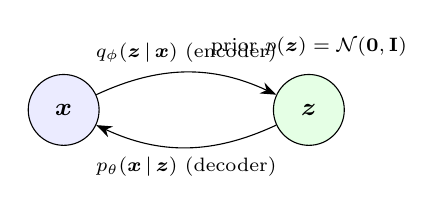
\begin{tikzpicture}[>={Stealth[length=2mm]},node distance=16mm,
  v/.style={draw,circle,minimum size=9mm,font=\small}]
  \node[v,fill=blue!8] (x) {$\x$};
  \node[v,fill=green!10,right=22mm of x] (z) {$\z$};
  \draw[->,bend left=25] (x) to node[above,font=\scriptsize]{$q_\phi(\z\given\x)$ (encoder)} (z);
  \draw[->,bend left=25] (z) to node[below,font=\scriptsize]{$p_\theta(\x\given\z)$ (decoder)} (x);
  \node[font=\scriptsize,above=1mm of z] {prior $p(\z)=\N(\bm0,\II)$};
\end{tikzpicture}
\caption{The VAE as a latent-variable model: an inference network
$q_\phi(\z\given\x)$ approximates the intractable posterior; a generative network
$p_\theta(\x\given\z)$ decodes.}
\label{fig:vae-graph}
\end{figure}

The prior is $p(\z)=\N(\bm0,\II)$. The encoder outputs a diagonal-Gaussian
posterior
\begin{equation}
q_\phi(\z\given\x)=\N\!\big(\z;\,\bm\mu_\phi(\x),\,\diag\bm\sigma_\phi^2(\x)\big),
\end{equation}
and the decoder defines $p_\theta(\x\given\z)$ (here a Gaussian observation model,
which makes the reconstruction term a weighted squared error; see
\S\ref{sec:vaeloss}).

\subsection{The VAE objective: ELBO decomposition}
Specialising \eqref{eq:elbo-jensen} and splitting the log-ratio,
\begin{align}
\mathcal L(\theta,\phi;\x)
&=\E_{q_\phi}\!\Big[\log p_\theta(\x\given\z)
   +\log p(\z)-\log q_\phi(\z\given\x)\Big]\\
&=\underbrace{\E_{q_\phi}\!\big[\log p_\theta(\x\given\z)\big]}_{\text{(i) reconstruction}}
  \;-\;\underbrace{\KL\!\big(q_\phi(\z\given\x)\,\|\,p(\z)\big)}_{\text{(ii) regulariser}} .
\label{eq:vae-elbo}
\end{align}
We \emph{maximise} $\mathcal L$, equivalently \emph{minimise} $-\mathcal L$. Term
(i) pulls reconstructions toward the data; term (ii) pulls the posterior toward
the prior and has the closed form of Lemma~\ref{lem:klgauss}:
\begin{equation}
\KL\!\big(q_\phi(\z\given\x)\,\|\,\N(\bm0,\II)\big)
=\frac12\sum_{j=1}^{d}\Big(\mu_{\phi,j}^2+\sigma_{\phi,j}^2-\log\sigma_{\phi,j}^2-1\Big).
\label{eq:vae-kl}
\end{equation}
Term (i) is estimated by a single reparameterised sample \eqref{eq:reparam}:
$\widehat{\mathcal L}_{\text{rec}}=\log p_\theta\big(\x\given \bm\mu_\phi+\bm\sigma_\phi\odot\eps\big)$.

\subsection{The practical reconstruction loss}
\label{sec:vaeloss}
A pure Gaussian likelihood gives $-\log p_\theta(\x\given\z)\propto\|\x-\hat\x\|_2^2$,
which over-smooths MRI. The code therefore uses a perceptually-weighted
reconstruction term plus the closed-form KL, with $\beta_{\mathrm{KL}}=10^{-6}$:
\begin{align}
\mathcal L_{\mathrm{VAE}}
&=\underbrace{\|\x-\hat\x\|_1}_{\ell_1}
+\;\lambda_{\mathrm{ms}}\big(1-\mathrm{MSSSIM}(\x,\hat\x)\big)
+\;\beta_{\mathrm{KL}}\,\KL\!\big(q_\phi\|\,p\big),\\
&\hspace{20mm}\lambda_{\mathrm{ms}}=0.5,\qquad \beta_{\mathrm{KL}}=10^{-6}.
\label{eq:vae-loss}
\end{align}
The tiny $\beta_{\mathrm{KL}}$ is a deliberate $\beta$-VAE choice: the latent must
\emph{retain reconstruction detail} for the downstream diffusion model, so we
barely regularise toward the prior (the $\times8$ bottleneck, not the prior, does
the compressing).

\paragraph{Structural similarity (the MS-SSIM term).}
Single-scale SSIM compares local luminance, contrast and structure of two images
through Gaussian-windowed local statistics $\mu,\sigma,\sigma_{xy}$:
\begin{equation}
\mathrm{SSIM}(\x,\hat\x)=
\frac{(2\mu_x\mu_{\hat x}+c_1)(2\sigma_{x\hat x}+c_2)}
     {(\mu_x^2+\mu_{\hat x}^2+c_1)(\sigma_x^2+\sigma_{\hat x}^2+c_2)},
\end{equation}
with stabilisers $c_1,c_2$. MS-SSIM evaluates the contrast--structure factor
across a $5$-level Gaussian pyramid (weights
$0.0448,0.2856,0.3001,0.2363,0.1333$) and multiplies them with the finest-scale
SSIM. Because $\mathrm{MSSSIM}\in[0,1]$ with $1$ = identical, $1-\mathrm{MSSSIM}$ is
a valid loss.

\subsection{Empirical latent scaling}
\label{sec:scaling}
A diffusion model expects unit-variance inputs. Rather than Stable Diffusion's
hard-coded $0.18215$ (specific to a natural-image VAE), we measure the standard
deviation of \emph{this} VAE's latents over $2000$ slices and rescale:
\begin{equation}
s=\frac{1}{\sigma_z},\qquad \sigma_z=\mathrm{std}\big(E_\phi(\x)\big)=0.7927
\;\;\Longrightarrow\;\; s=1.262,
\label{eq:scaling}
\end{equation}
so the diffusion model operates on $\z_0=s\,E_\phi(\x)$ with
$\Var(\z_0)\approx s^2\sigma_z^2=1$ (property G1). At decode time we undo it:
$\hat\x=D_\psi(\hat\z_0/s)$.

% ---------------------------------------------------------------------------
\section{DDPM on the healthy latent manifold}
\label{sec:ddpm}
% ---------------------------------------------------------------------------
\textbf{Implementation.} A \texttt{diffusers} UNet ($89.54$\,M params; block widths
$128,256,384,512$; in/out $=4$ channels; sample size $32$) trained with $\eps$-
prediction over $T=1000$ steps on the cosine schedule
(\texttt{squaredcos\_cap\_v2}, $\beta\in[10^{-4},2\!\times\!10^{-2}]$), EMA decay
$0.999$, gradient clip $1.0$.

\begin{figure}[h!]
\centering
\resizebox{\textwidth}{!}{%
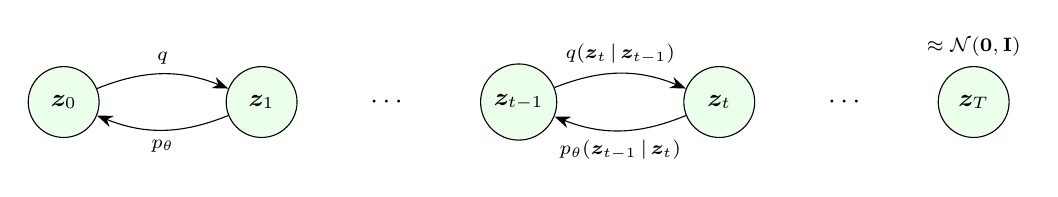
\begin{tikzpicture}[>={Stealth[length=2mm]},node distance=16mm,
  v/.style={draw,circle,minimum size=9mm,font=\small,fill=green!8}]
  \node[v] (z0) {$\z_0$};
  \node[v,right=of z0] (z1) {$\z_1$};
  \node[right=8mm of z1] (d1) {$\cdots$};
  \node[v,right=8mm of d1] (zt1) {$\z_{t-1}$};
  \node[v,right=of zt1] (zt) {$\z_t$};
  \node[right=8mm of zt] (d2) {$\cdots$};
  \node[v,right=8mm of d2] (zT) {$\z_T$};
  \draw[->,bend left=22] (z0) to node[above,font=\scriptsize]{$q$} (z1);
  \draw[->,bend left=22] (zt1) to node[above,font=\scriptsize]{$q(\z_t\given\z_{t-1})$} (zt);
  \draw[->,bend left=22] (zt) to node[below,font=\scriptsize]{$p_\theta(\z_{t-1}\given\z_t)$} (zt1);
  \draw[->,bend left=22] (z1) to node[below,font=\scriptsize]{$p_\theta$} (z0);
  \node[font=\scriptsize,above=0mm of zT]{$\approx\N(\bm0,\II)$};
\end{tikzpicture}}
\caption{Forward (top, fixed Gaussian) and reverse (bottom, learned) Markov chains
on the scaled healthy latent $\z_0$.}
\label{fig:chain}
\end{figure}

\subsection{Forward process and the diffusion kernel}
The forward chain adds Gaussian noise with variance schedule $\{\beta_t\}$:
\begin{equation}
q(\z_t\given\z_{t-1})=\N\!\big(\z_t;\,\sqrt{1-\beta_t}\,\z_{t-1},\,\beta_t\II\big).
\label{eq:fwd}
\end{equation}
\begin{theorem}[Diffusion kernel]\label{thm:kernel}
With $\alpha_t=1-\beta_t$ and $\abar_t=\prod_{s=1}^t\alpha_s$,
\begin{equation}
q(\z_t\given\z_0)=\N\!\big(\z_t;\,\sqrt{\abar_t}\,\z_0,\,(1-\abar_t)\II\big),
\qquad
\z_t=\sqrt{\abar_t}\,\z_0+\sqrt{1-\abar_t}\,\eps.
\label{eq:kernel}
\end{equation}
\end{theorem}
\begin{proof}
One step in reparameterised form (property G1) is
$\z_t=\sqrt{\alpha_t}\,\z_{t-1}+\sqrt{1-\alpha_t}\,\eps_{t-1}$. Substitute the same
expression for $\z_{t-1}$:
\begin{align}
\z_t&=\sqrt{\alpha_t}\Big(\sqrt{\alpha_{t-1}}\,\z_{t-2}+\sqrt{1-\alpha_{t-1}}\,\eps_{t-2}\Big)
      +\sqrt{1-\alpha_t}\,\eps_{t-1}\\
   &=\sqrt{\alpha_t\alpha_{t-1}}\,\z_{t-2}
     +\underbrace{\sqrt{\alpha_t(1-\alpha_{t-1})}\,\eps_{t-2}
     +\sqrt{1-\alpha_t}\,\eps_{t-1}}_{\text{independent Gaussians}}.
\end{align}
By property G2 the two noise terms merge into one zero-mean Gaussian with variance
\begin{equation}
\alpha_t(1-\alpha_{t-1})+(1-\alpha_t)=1-\alpha_t\alpha_{t-1},
\end{equation}
so $\z_t=\sqrt{\alpha_t\alpha_{t-1}}\,\z_{t-2}+\sqrt{1-\alpha_t\alpha_{t-1}}\,\bar\eps$.
Inducting down to $\z_0$ turns the product into $\abar_t$ and the variance into
$1-\abar_t$, proving \eqref{eq:kernel}.
\end{proof}

\noindent The \emph{signal-to-noise ratio} $\mathrm{SNR}(t)=\abar_t/(1-\abar_t)$
determines which structures survive to step $t$ (Fig.~\ref{fig:schedule},
Table~\ref{tab:snr}); it underpins the choice of the partial-noise level
(\S\ref{sec:partial}).

\begin{figure}[h!]
\centering

\includegraphics[width=\textwidth]{figures/fig_schedule.png}
\caption{Cosine-schedule coefficients (left) and SNR in dB (right) for $T=1000$,
computed from the exact \texttt{squaredcos\_cap\_v2} schedule. The operating level
$T_{\mathrm{int}}=300$ and the multi-scale set $\{100,250,400\}$ are marked.}
\label{fig:schedule}
\end{figure}

\begin{table}[h!]
\centering\small
\caption{Exact schedule values at the project's operating timesteps.}
\label{tab:snr}
\begin{tabular}{@{}rcccc@{}}
\toprule
$t$ & $\abar_t$ & $\sqrt{\abar_t}$ (signal) & $\sqrt{1-\abar_t}$ (noise) & SNR \\
\midrule
100 & 0.9716 & 0.986 & 0.169 & $34.2$ ($+15.3$\,dB)\\
250 & 0.8459 & 0.920 & 0.393 & $5.49$ ($+7.4$\,dB)\\
\textbf{300} & \textbf{0.7856} & \textbf{0.886} & \textbf{0.463} & $\mathbf{3.67}$ ($+5.6$\,dB)\\
400 & 0.6460 & 0.804 & 0.595 & $1.83$ ($+2.6$\,dB)\\
\bottomrule
\end{tabular}
\end{table}

\paragraph{Cosine schedule.} (Nichol \& Dhariwal, 2021)
\begin{equation}
\abar_t=\frac{f(t)}{f(0)},\quad
f(t)=\cos^2\!\Big(\frac{t/T+s}{1+s}\cdot\frac{\pi}{2}\Big),\quad
\beta_t=1-\frac{\abar_t}{\abar_{t-1}}.
\end{equation}

\subsection{Reverse process and the variational bound}
The reverse chain is learned as $p_\theta(\z_{t-1}\given\z_t)=\N(\bm\mu_\theta(\z_t,t),\sigma_t^2\II)$
with $p(\z_T)=\N(\bm0,\II)$. Applying the ELBO to the whole chain and decomposing,
\begin{align}
\E_q\!\big[-\log p_\theta(\z_0)\big]
&\le \E_q\!\Big[-\log\frac{p_\theta(\z_{0:T})}{q(\z_{1:T}\given\z_0)}\Big]\\
&=\E_q\Big[\KL\!\big(q(\z_T\given\z_0)\|p(\z_T)\big)
   -\log p_\theta(\z_0\given\z_1)\notag\\
&\hspace{12mm}
   +\sum_{t=2}^{T}\KL\!\big(q(\z_{t-1}\given\z_t,\z_0)\,\|\,p_\theta(\z_{t-1}\given\z_t)\big)\Big].
\label{eq:diff-elbo}
\end{align}
The decomposition uses Bayes' rule
$q(\z_t\given\z_{t-1})=\frac{q(\z_{t-1}\given\z_t,\z_0)\,q(\z_t\given\z_0)}{q(\z_{t-1}\given\z_0)}$
and a telescoping of the $q(\cdot\given\z_0)$ factors. The first term has no
parameters; the work is the per-step $\KL$.

\subsection{The tractable posterior}
\begin{theorem}[Forward posterior]\label{thm:posterior}
\begin{equation}
q(\z_{t-1}\given\z_t,\z_0)=\N\!\big(\z_{t-1};\,\tilde{\bm\mu}_t,\,\tilde\beta_t\II\big),
\end{equation}
\begin{align}
\tilde\beta_t&=\frac{1-\abar_{t-1}}{1-\abar_t}\,\beta_t,\\
\tilde{\bm\mu}_t(\z_t,\z_0)&=
\frac{\sqrt{\abar_{t-1}}\,\beta_t}{1-\abar_t}\,\z_0
+\frac{\sqrt{\alpha_t}\,(1-\abar_{t-1})}{1-\abar_t}\,\z_t.
\label{eq:posterior}
\end{align}
\end{theorem}
\begin{proof}
By Bayes, $q(\z_{t-1}\given\z_t,\z_0)\propto q(\z_t\given\z_{t-1})\,q(\z_{t-1}\given\z_0)$,
a product of the Gaussians \eqref{eq:fwd} and \eqref{eq:kernel}. Their exponent,
as a function of $\z_{t-1}$, is
\begin{align}
-\frac12\Big[&\frac{\|\z_t-\sqrt{\alpha_t}\z_{t-1}\|^2}{\beta_t}
   +\frac{\|\z_{t-1}-\sqrt{\abar_{t-1}}\z_0\|^2}{1-\abar_{t-1}}\Big]\\
=-\frac12\Big[&\Big(\tfrac{\alpha_t}{\beta_t}+\tfrac{1}{1-\abar_{t-1}}\Big)\|\z_{t-1}\|^2
  -2\,\z_{t-1}^\top\bm b +\text{const}\Big],
\end{align}
with $\bm b=\frac{\sqrt{\alpha_t}}{\beta_t}\z_t+\frac{\sqrt{\abar_{t-1}}}{1-\abar_{t-1}}\z_0$.
Property G3 (completing the square) gives precision
\begin{equation}
\tilde\beta_t^{-1}=\frac{\alpha_t}{\beta_t}+\frac{1}{1-\abar_{t-1}}
=\frac{\alpha_t(1-\abar_{t-1})+\beta_t}{\beta_t(1-\abar_{t-1})}
=\frac{1-\abar_t}{\beta_t(1-\abar_{t-1})},
\end{equation}
using $\alpha_t(1-\abar_{t-1})+\beta_t=\alpha_t-\abar_t+\beta_t=1-\abar_t$. The mean
is $\tilde{\bm\mu}_t=\tilde\beta_t\,\bm b$, which expands to \eqref{eq:posterior}.
\end{proof}

\subsection{From KL to mean-matching to noise prediction}
Because $p_\theta$ and the posterior share covariance $\sigma_t^2\II$, the per-step
KL reduces (Lemma~\ref{lem:klgauss}, $\bm\mu$-only terms) to
\begin{equation}
L_{t-1}=\E_q\!\Big[\tfrac{1}{2\sigma_t^2}\,\|\tilde{\bm\mu}_t-\bm\mu_\theta(\z_t,t)\|^2\Big]+\text{const}.
\label{eq:meanmatch}
\end{equation}
Now reparameterise. Invert \eqref{eq:kernel}:
$\z_0=\frac{1}{\sqrt{\abar_t}}\big(\z_t-\sqrt{1-\abar_t}\,\eps\big)$. Substitute into
$\tilde{\bm\mu}_t$ \eqref{eq:posterior} and simplify (the $\z_t$ coefficients combine):
\begin{align}
\tilde{\bm\mu}_t
&=\frac{\sqrt{\abar_{t-1}}\,\beta_t}{1-\abar_t}\cdot
   \frac{\z_t-\sqrt{1-\abar_t}\,\eps}{\sqrt{\abar_t}}
  +\frac{\sqrt{\alpha_t}\,(1-\abar_{t-1})}{1-\abar_t}\,\z_t\\
&=\frac{1}{\sqrt{\alpha_t}}\Big(\z_t-\frac{\beta_t}{\sqrt{1-\abar_t}}\,\eps\Big).
\label{eq:mu-eps}
\end{align}
Choosing $\bm\mu_\theta$ with the \emph{same} form but $\eps_\theta$ in place of
$\eps$, the mean gap becomes a noise gap:
\begin{equation}
\|\tilde{\bm\mu}_t-\bm\mu_\theta\|^2
=\frac{\beta_t^2}{\alpha_t(1-\abar_t)}\,\|\eps-\eps_\theta(\z_t,t)\|^2.
\end{equation}
Hence
\begin{equation}
L_{t-1}=\E_{\z_0,\eps}\!\Big[\tfrac{\beta_t^2}{2\sigma_t^2\alpha_t(1-\abar_t)}\,
\|\eps-\eps_\theta(\z_t,t)\|^2\Big].
\label{eq:Lt}
\end{equation}
Dropping the per-$t$ weight (Ho et al.\ 2020, which improves samples) gives the
objective the code optimises over \emph{healthy} latents:
\begin{equation}
\boxed{\;
\mathcal L_{\mathrm{simple}}(\theta)=
\E_{\z_0,\;t\sim\mathcal U\{1,\dots,T\},\;\eps\sim\N(\bm0,\II)}
\Big[\big\|\eps-\eps_\theta\!\big(\sqrt{\abar_t}\z_0+\sqrt{1-\abar_t}\eps,\,t\big)\big\|_2^2\Big].
\;}
\label{eq:simple}
\end{equation}
On the project's $30$-patient pilot this reached a best validation
$\mathcal L_{\mathrm{simple}}=0.411$ at epoch $8$ (EMA weights).

% ---------------------------------------------------------------------------
\section{DDIM partial-noise reconstruction}
\label{sec:ddim}
% ---------------------------------------------------------------------------
\subsection{Deterministic sampler}
DDIM (Song et al.\ 2021) defines a family of non-Markovian processes with the
\emph{same} marginals \eqref{eq:kernel}, indexed by stochasticity $\sigma_t\ge0$:
\begin{align}
q_\sigma(\z_{t-1}\given\z_t,\z_0)=\N\Big(
&\sqrt{\abar_{t-1}}\,\z_0\notag\\
&+\sqrt{1-\abar_{t-1}-\sigma_t^2}\;\frac{\z_t-\sqrt{\abar_t}\,\z_0}{\sqrt{1-\abar_t}},
\;\sigma_t^2\II\Big).
\end{align}
Since \eqref{eq:simple} is unchanged, we reuse $\eps_\theta$. Define the predicted
clean latent
\begin{equation}
\hat{\z}_0(\z_t,t)=\frac{\z_t-\sqrt{1-\abar_t}\,\eps_\theta(\z_t,t)}{\sqrt{\abar_t}},
\label{eq:z0hat}
\end{equation}
giving the generative update
\begin{align}
\z_{t-1}=\;&\sqrt{\abar_{t-1}}\,\hat{\z}_0(\z_t,t)\notag\\
&+\sqrt{1-\abar_{t-1}-\sigma_t^2}\;\eps_\theta(\z_t,t)+\sigma_t\,\eps.
\label{eq:ddim}
\end{align}
Setting $\sigma_t=0$ makes the map \textbf{deterministic}, so reconstructions are
reproducible up to the single injected noise vector. The code runs $\le 50$ DDIM
steps inside $[0,T_{\mathrm{int}}]$ ($\approx 20\times$ faster than $1000$ steps,
exact for the marginals).

\subsection{Partial noising and the counterfactual}
\label{sec:partial}
At inference we noise only to $T_{\mathrm{int}}=300$, then denoise:
\begin{equation}
\z_{T_{\mathrm{int}}}=\sqrt{\abar_{300}}\,\z_0+\sqrt{1-\abar_{300}}\,\eps
=0.886\,\z_0+0.463\,\eps,
\end{equation}
i.e.\ $88.6\%$ signal is retained at SNR $+5.6$\,dB (Table~\ref{tab:snr}) ---
enough corruption to erase localised pathology, little enough to keep
patient-specific healthy anatomy. Iterating \eqref{eq:ddim} from $300\to0$ yields
$\hat{\z}_0^{\mathrm{healthy}}$, decoded to
\begin{equation}
\hat\x=D_\psi\!\big(\hat{\z}_0^{\mathrm{healthy}}/s\big).
\end{equation}
\paragraph{Why anomalies heal (manifold view).} Let $\mathcal M_h$ be the support
of the learned healthy latent distribution. Write a test latent as
$\z_0=\z_h+\bm a$ with $\z_h\in\mathcal M_h$ and $\bm a$ the lesion component.
Adding noise of std $0.463$ at $T_{\mathrm{int}}$ destroys components whose energy
lies in the corrupted band; the reverse chain --- trained only on $\mathcal M_h$
--- denoises toward $\mathcal M_h$, returning $\hat\z_0\approx\z_h$ and erasing
$\bm a$. The residual $|\x-\hat\x|\approx|\bm a|$ thus localises the lesion. This
is precisely a \emph{counterfactual}: ``what this slice would look like if
healthy.''

% ---------------------------------------------------------------------------
\section{Scoring, calibration and metrics}
\label{sec:score}
% ---------------------------------------------------------------------------
\subsection{Modality-weighted residual with the CE channel}
With normalised input $\x$ and reconstruction $\hat\x$, the per-channel residual is
$r_k=|\x_k-\hat\x_k|$, $k\in\{t1n,t1c,t2w,t2f\}$, plus a contrast-enhancement
channel
\begin{equation}
r_{\mathrm{CE}}=\big|(\x_{t1c}-\x_{t1n})-(\hat\x_{t1c}-\hat\x_{t1n})\big|.
\end{equation}
Each is corrected by a healthy baseline $M_k$ (\S\ref{sec:calib}), rectified, and
combined with clinical-salience weights $\bm w\propto(0.5,1.0,0.75,1.5)$,
$w_{\mathrm{CE}}=1$:
\begin{align}
A_{\mathrm{pix}}(\bm u)=\Big(\sum_{k}\bar w_k\,\max(r_k(\bm u)-M_k(\bm u),0)\Big)
\,\mathbb 1[\bm u\in\Omega],\quad \bar w_k=\tfrac{w_k}{\sum_j w_j},
\end{align}
over the eroded brain mask $\Omega$.

\subsection{Latent residual and dual-space fusion}
A complementary latent residual
$A_{\mathrm{lat}}=\mathrm{Up}\big(\tfrac1C\sum_c|\z_{0,c}-\hat\z_{0,c}|\big)$ is
fused after standardising each map by its healthy scale $s_{\mathrm{pix}},s_{\mathrm{lat}}$:
\begin{equation}
A(\bm u)=\frac{A_{\mathrm{pix}}(\bm u)}{s_{\mathrm{pix}}}
+\alpha\,\frac{A_{\mathrm{lat}}(\bm u)}{s_{\mathrm{lat}}},\qquad \alpha=0.5.
\label{eq:fusion}
\end{equation}
The score is optionally aggregated over $T\in\{100,250,400\}$ (the multi-scale set
of Table~\ref{tab:snr}) by the mean: $A^{\mathrm{multi}}=\tfrac13\sum_T A^{(T)}$.

\subsection{Healthy-set calibration}
\label{sec:calib}
On held-out healthy slices we estimate the baseline $M_k$ (mean residual over
healthy tissue), the fusion scales, and the operating threshold as a high
percentile of pooled healthy brain-voxel scores:
\begin{equation}
\tau=\mathrm{Percentile}_{95}\big(\{A(\bm u):\bm u\in\Omega,\ \x\ \text{healthy}\}\big),
\quad \hat P(\bm u)=\mathbb 1[A(\bm u)>\tau].
\end{equation}
By construction $\tau$ passes only the top $5\%$ of healthy voxels --- a controlled,
label-free false-positive rate. As an order statistic (Wilks, 1941),
$\sim\!20/\alpha=400$ samples suffice; the code uses up to $200$ slices
($\sim\!10^6$ voxels).

\subsection{Evaluation metrics}
\begin{align}
\mathrm{AUROC}&=\Pr\big(A(\bm u_+)>A(\bm u_-)\big)=\int_0^1\!\mathrm{TPR}\,\dd\,\mathrm{FPR},\\
\mathrm{Dice}(\hat P,G)&=\frac{2|\hat P\cap G|}{|\hat P|+|G|}
=\frac{2\,\mathrm{TP}}{2\,\mathrm{TP}+\mathrm{FP}+\mathrm{FN}}.
\end{align}
AUROC/AUPRC are threshold-free (ranking quality); Dice is reported at the
calibrated $\tau$, the best-global threshold, and the per-slice oracle, whose
spread separates \emph{score} error from \emph{threshold} error. On the pilot the
system reached slice-level AUROC $\approx0.86\text{--}0.94$ with low calibrated
Dice, diagnostic of an edge-artefact-dominated residual rather than a detection
failure.

% ---------------------------------------------------------------------------
\section*{Reading the numbers (summary)}
\addcontentsline{toc}{section}{Reading the numbers (summary)}
% ---------------------------------------------------------------------------
\begin{itemize}[leftmargin=1.4em]
\item \textbf{VAE loss} mixes $\ell_1$, $1-\mathrm{MSSSIM}\in[0,1]$ and a
$10^{-6}$-scaled KL; the KL term is intentionally negligible so the latent keeps
detail. A clean VAE shows small interior residual but a bright skull/edge rim ---
the artefact the baseline $M_k$ must absorb.
\item \textbf{Diffusion loss} \eqref{eq:simple} is an $\eps$-MSE on unit-variance
noise, so a do-nothing predictor scores $\approx1.0$; the pilot's best
val $0.411$ means the UNet explains $\approx 59\%$ of the injected-noise variance.
Validation \emph{below} training is the healthy (non-overfit) regime.
\item \textbf{$T_{\mathrm{int}}=300$} keeps $88.6\%$ signal (Table~\ref{tab:snr});
smaller $T$ misses large lesions, larger $T$ erases healthy detail --- hence the
multi-scale set $\{100,250,400\}$.
\item \textbf{AUROC vs.\ Dice}: high AUROC + low calibrated Dice $\Rightarrow$ the
score ranks lesions correctly but a single global $\tau$ cannot separate them from
the edge rim; the oracle$-$calibrated Dice gap quantifies the threshold headroom.
\end{itemize}

\section*{Key references}
\addcontentsline{toc}{section}{Key references}
\begin{enumerate}[label={[\arabic*]},leftmargin=2.2em,itemsep=1pt]
\item Kingma, Welling (2014). \textit{Auto-Encoding Variational Bayes}. ICLR.
\item Higgins et al.\ (2017). \textit{$\beta$-VAE}. ICLR.
\item Rombach et al.\ (2022). \textit{High-Resolution Image Synthesis with Latent Diffusion Models}. CVPR.
\item Ho, Jain, Abbeel (2020). \textit{Denoising Diffusion Probabilistic Models}. NeurIPS.
\item Song, Meng, Ermon (2021). \textit{Denoising Diffusion Implicit Models}. ICLR.
\item Nichol, Dhariwal (2021). \textit{Improved DDPMs}. ICML.
\item Wang, Simoncelli, Bovik (2003). \textit{Multiscale Structural Similarity}. Asilomar.
\item Wyatt et al.\ (2022). \textit{AnoDDPM}. CVPR-W.
\item Baur et al.\ (2021). \textit{Autoencoders for Unsupervised Anomaly Segmentation in Brain MR}. MedIA.
\item Wilks (1941). \textit{Determination of Sample Sizes for Setting Tolerance Limits}. Ann.\ Math.\ Stat.
\end{enumerate}

\end{document}
